Proteins are complex macromolecules that lie the foundation for all life on Earth. From providing structural support to cells and tissues through proteins like collagen and keratin, to acting as catalysts for chemical reactions such as the digestion of starch, proteins maintain the normal functioning of living organisms. Since they are fundamental to so many biological processes that make life possible, it is no wonder that the malfunction of proteins can have devastating effects on the health of individuals. To take one example, Parkinson's disease, a chronic degenerative disease that affects the motor system in humans, arises as a result of the aggregation of alpha-sinuclein protein in the brain, a molecule that regulates synaptic vesicle trafficking and subsequent neurotransmitter release.

\section{Computational protein engineering}
Protein engineering is a field of biotechnology that aims to artificially modify existing proteins in order to enhance their properties or create new functions. The field also looks at ways to cure diseases that are the result of malfunctioning biological processes and proteins. For example, as early as 1988, \citet{insulin} induced mutations into the insulin agents used to treat diabetes in order to make them easier to be absorbed by the body and better mimic the action of the naturally-produced insulin hormone. 

Albeit it is a promising field, protein engineering can be a costly, labour intensive process in which researchers have to first determine the mutations most likely to be successful for the task at hand and then experimentally validate them. \textit{Computational protein engineering} aims to optimise the exploratory process by using computational methods to accelerate the generation of the mutations that are most likely to be successful. 

In recent years, pre-trained machine learning (ML) models have garnered significant attention in the field of protein representation. Notably, models have been developed to deal with both the sequence and structure modalities of proteins \cite{ESM, prottrans, gearnet}. These models have demonstrated their potential in various applications such as protein fitness\footnote{Fitness indicates how much better a mutation is compared to the original protein. Fitness is a general concept, and can mean different things depending on the context.} prediction \cite{ESM-1v, tranception}. They are usually employed in a ``zero-shot'' manner, meaning that they make predictions on data they have never seen or been explicitly trained on.
Their success has also shown promising experimental results in protein engineering  \cite{mutcompute, Lu2022}.

Present state-of-the-art methods for predicting mutation fitness use sequence data, as this data has been historically more readily available: large language models are pre-trained on millions of sequences and then used to aid the discovery process. However, the last few years have seen a major breakthrough in protein structure prediction through the AlphaFold2 program developed by DeepMind \cite{alphafold}. AlphaFold2 is now routinely used to predict the structure of proteins from their sequence, so the corpus of structural information about proteins has more than doubled \cite{portapardo2022structural}.

In this context, structure-based models have been proven experimentally successful, particularly those pre-trained on predicting amino acid residues based on local atomic environments. Recently, \citet{Lu2022} have engineering plastic decomposing enzymes to be more thermally stable using a structure model based on 3D-Convolutional Neural Networks (3D-CNNs). Despite their success, these structural models have not been systematically compared with sequence-based models using the same benchmarking datasets. 

This project aims to fill this \textbf{research gap} by proposing a novel approach to structure-based protein engineering through the usage of equivariant graph neural networks, and then comparing this approach to the most important representatives of the sequence-based method. 

\section{Equivariant graph neural networks}
I propose a novel approach to mutation generation for proteins through the usage of graph neural networks (GNNs). While structural methods have so far employed 3D-CNNs, this approach has limitations: firstly, because CNNs operate on grid-like data, protein structures must be voxelised\footnote{Voxelisation is the process of converting data structures that store geometric information in a continuous domain (such as a 3D triangular mesh) into a rasterised image (a discrete grid).} into cubes, thereby losing some of their geometric attributes; secondly, voxelised structures are harder to be combined with sequence-based models in a principled way. In contrast, the advances made in the field of GNNs now allows us to process geometric graphs without any loss in detail and information.

Graph neural networks have gained popularity in the last couple of years and have become the most promising machine learning technique for processing graph information. All GNNs use some form of \textit{neural message passing}, where messages are exchanged between nodes and updated using a neural network \citep{gilmer2017neural}. Advances in this field have led to the development of \textbf{equivariant graph neural networks}. This type of GNNs can process information while preserving the structural properties of node features, like equivariance or invariance to \textit{3D translations} and \textit{rotations}.

Protein structures can be represented as graphs with nodes corresponding to atoms. Each atom's scalar feature is its atom type (e.g., Carbon, Nitrogen, Hydrogen, etc.) and its vector feature is the atom's position in 3D space. Using this representation, researchers can design and train EGNNs to perform a range of molecular tasks. This approach has been proven successful on the scoring of protein-ligand complexes \cite{egnn-application-1} or model quality assessment (MQA) \cite{gvp1}.

\section{Unsupervised EGNNs for mutation generation}

The original aim of this project was to evaluate the performance of a handful of newly proposed EGNN architectures to the molecular task of amino acid residue identity prediction, here reffered to as the RES task \cite{atom-3d}. This task involves training an ML model to predict the missing amino acid in a protein given the surrounding atoms.

\textbf{I extend} the original scope of the project to use these trained EGNN models to propose single-point mutations given a protein structure, thereby putting to use the biophysical knowledge that these models have inferred from training on the RES task. These models effectively act as \textbf{unsupervised} models for predicting the fitness of a mutated protein, such as the protein's thermostability, toxicity, fluorescence, etc. The idea behind my approach is to use the trained EGNN models to score the viability of each amino acid in a protein sequence. For example, by targeting each position of an amino acid sequence in turn, I observe the positions at which the EGNN model is \textit{least confident}. This could be an indication that the position is a good candidate for mutations. Figure \ref{idea} illustrates this concept visually.

\begin{figure}[!h]
    \centering
    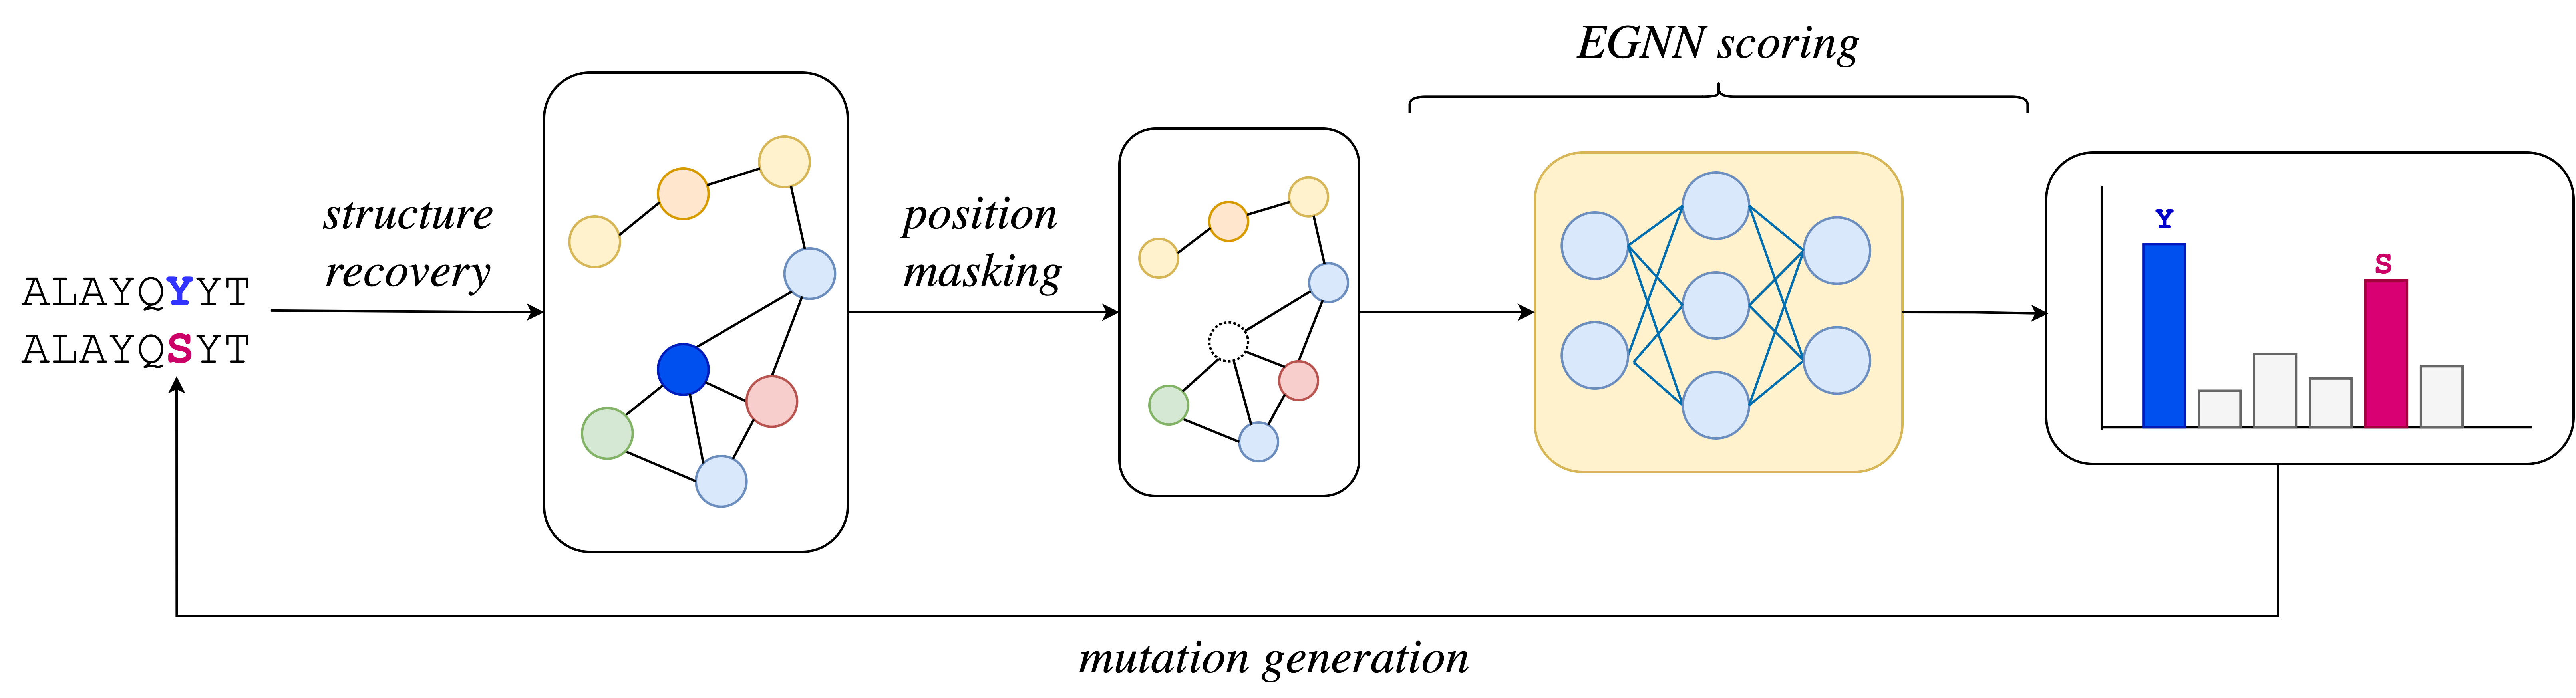
\includegraphics[width=\textwidth]{masters-report/figures/pipeline-4.png}
    \caption{For every sequence I recover its structure and mask each amino acid in turn. I pass the masked graph through a pre-trained EGNN model to recover the scores of every amino acid, which I then rank.  The key idea is that this pre-training allows the model to identify amino acids which seem “unusual” given their local environment and propose better fitting candidates instead.}
    \label{idea}
\end{figure}

The project will compare a couple of systematic approaches for extracting the candidate mutations by looking at the models' confidence when dealing with amino acids at targeted positions. 

\section{Augmented linear models for fitness prediction}

Having powerful, yet unsupervised models aids the exploratory process when dealing with new proteins – this project acts as a proof-of-concept to how EGNNs can become tools that help researchers accelerate the study of new proteins. Conversely, when data about a mutated sequence's fitness is already available to some extent, I can combine it with pre-trained models in order to create predictors that effectively operate in a \textbf{low-data regime} and take full advantage of both the latent knowledge of the unsupervised model and the task-specific information provided by the already existing, albeit limited, data. 

To this extent, I propose an \textbf{augmented} ridge regression model that learns to predict the protein fitness of single-point mutated sequences by combining the information about the amino acid present at each position with the EGNN score for the specified mutation. Although the usage of regression models for fitness prediction was first studied by \citet{chloe-hsu}, I extend and evaluate this approach to pre-trained EGNNs and find that it outperforms state-of-the-art transformer models when predicting the fitness of better-than-wildtype sequences. 

\section{Contributions}

This project aims to provide insights into the performance and suitability of EGNNs in protein engineering, specifically in the context of predictions based on the local atomic environment. My contributions are as follows:
\begin{itemize}
    \item I apply the most successful pre-training approach for structural methods \cite{mutcompute} to equivariant GNNs by using the ATOM3D RES dataset \cite{atom-3d} for residue identity prediction  (Section \ref{sec:res-task});
    \item I benchmark the resulting structure-based pre-trained models with the most successful zero-shot sequence-based approaches (Section \ref{sec:mutation-generation-results}). I observe that structure is competitive to sequence in downstream tasks when used in this way, although the amount of available structures used during pre-training is significantly lower than the number of sequences used in training sequence-based models;
    \item I extend the simple combination approach for assay labelled data and pre-trained model outputs \cite{chloe-hsu} to the structure pre-trained domain. I find the same general trends as \citet{chloe-hsu}: assay-labelled data quickly allows us to surpass zero-shot pre-trained sequence-based models with at few as 100 datapoints (Section \ref{sec:protein-fitness-prediction}).
\end{itemize}
